\documentclass[a4paper, 12pt]{article}
\usepackage[a4paper,top=1.5cm, bottom=1.5cm, left=1cm, right=1cm]{geometry}
\usepackage{cmap}					
\usepackage{mathtext} 				
\usepackage[T2A]{fontenc}			
\usepackage[utf8]{inputenc}			
\usepackage[english,russian]{babel}
\usepackage{multirow}
\usepackage{graphicx}
\usepackage{wrapfig}
\usepackage{tabularx}
\usepackage{float}
\usepackage{longtable}
\usepackage{hyperref}
\hypersetup{colorlinks=true,urlcolor=blue}
\usepackage[rgb]{xcolor}
\usepackage{amsmath, amsfonts, amssymb, amsthm, mathtools} 
\usepackage{icomma} 
\usepackage{euscript}
\usepackage{mathrsfs}
\usepackage{enumerate}
\usepackage{caption}
\usepackage{enumerate}
\mathtoolsset{showonlyrefs=true}
\usepackage{graphicx}
\usepackage{caption}
\usepackage{subcaption}
\usepackage{amsthm}
\usepackage[europeanresistors, americaninductors]{circuitikz}
\DeclareMathOperator{\sgn}{\mathop{sgn}}
\newcommand*{\hm}[1]{#1\nobreak\discretionary{}
	{\hbox{$\mathsurround=0pt #1$}}{}}

\title{\textbf{Определение теплоёмкости твёрдых тел (2.1.4)}}
\author{Манро Эйден}
\date{}

\begin{document}

\maketitle

\begin{center}
    \section*{Введение}
\end{center}

    \textbf{Цель работы:} 1) измерение количества подведенного тепла и вызванного им нагрева твердого тела; 2) определение теплоемкости по экстраполяции отношения $\Delta Q / \Delta T$ к нулевым потерям тепла.

    \bigskip

    \textbf{Оборудование:} калориметр с нагревателем и термометром сопротивления; амперметр; вольтметр; мост постоянного тока; источник питания 36 В.

    \bigskip

\begin{center}
    \section*{Теоретические сведения}
\end{center}

В данной работе происходит измерение теплоемкости твердого тела с использованием следующей принципиальной связи:
	
\bigskip

\begin{equation} \label{first_eq_of_thermal_capacity}
	C = \frac{\Delta Q}{\Delta T}
\end{equation} 

\bigskip

Определение количества теплоты, переданного телу вызывает некоторые затруднения, так как часть теплоты будет передана окружающей среде через стенки калориметра. В итоге, количество теплоты, переданное телу с учетом теплопотерь через стенки можно определить как:

\bigskip

\begin{equation} \label{termal_with_heat_lossing}
	\Delta Q = P\Delta t - \lambda \left( T - T_{\text{к}} \right) \Delta t,

\end{equation}

\bigskip

где $P$ -- мощность нагревателя, $\lambda$ -- коэффициент теплоотдачи стенок калориметра, $T$ -- температура тела, $T_{\text{к}}$ -- температура окружающего калориметр воздуха, $\Delta t$ -- время, в течении которого происходит нагрев.
 
Из уравнений (\ref{eq:first_eq_of_thermal_capacity}) и (\ref{eq:second_eq_of_thremal_capacity}) получаем:

\bigskip

\begin{equation} \label{second_eq_of_thremal_capacity}
    C = \frac{P - \lambda \left(T - T_{\text{к}} \right) }{\Delta T /\Delta t}
\end{equation}

\bigskip

Формула \eqref{second_eq_of_thremal_capacity} является основной расчетной формулой данной работы.

В формуле \eqref{second_eq_of_thremal_capacity} в знаменателе стоит величина, для определения которой воспользуемся следующей методикой:

Построим график зависимости $\displaystyle \frac{\Delta T}{\Delta t} = f \left( T \right)$ для широкого диапазона температур, после чего экстраполируем его для значения $T = T_{\text{к}}$. В таком случае формула (\ref{eq:second_eq_of_thremal_capacity}) приобретает вид:

\bigskip

\begin{equation}
	C = \frac{P}{\left( \Delta T / \Delta t \right)_{T_{\text{к}}}}
	\label{final_eq_for_capacity}
\end{equation}

\bigskip

Измерение температуры строится на принципе линейной зависимости сопротивления материала от изменения температуры по закону:

\bigskip

\begin{equation}
	R_{T} = R_{0} \left( 1 + \alpha \Delta T \right),
\end{equation}

\bigskip

Где $R_{0}$ -- сопротивление термометра при температуре $0^\circ$C, $R_{T}$ -- сопротивление термометра при данной температуре. Учитывая данную зависимость, получаем итоговый вид для основной формулы:

\bigskip

\begin{equation}
	C = \frac{PR\alpha}{\left( \frac{dR}{dt} \right)_{T_{\text{к}}}\left( 1 + \alpha \Delta T_{\text{К}} \right)}
	\label{capacity}
\end{equation}

\bigskip

Коэффициент $\alpha$, входящий в данную формулу для меди равен $\alpha = 4,28 \cdot 10^{-3} \, K^{-1}$, все остальные величины определяются экспериментально.

\bigskip

\subsection*{Экспериментальная установка}

\begin{wrapfigure}[9]{r}{0.3\textwidth}
\vspace{-2.5ex}
	\begin{center}
		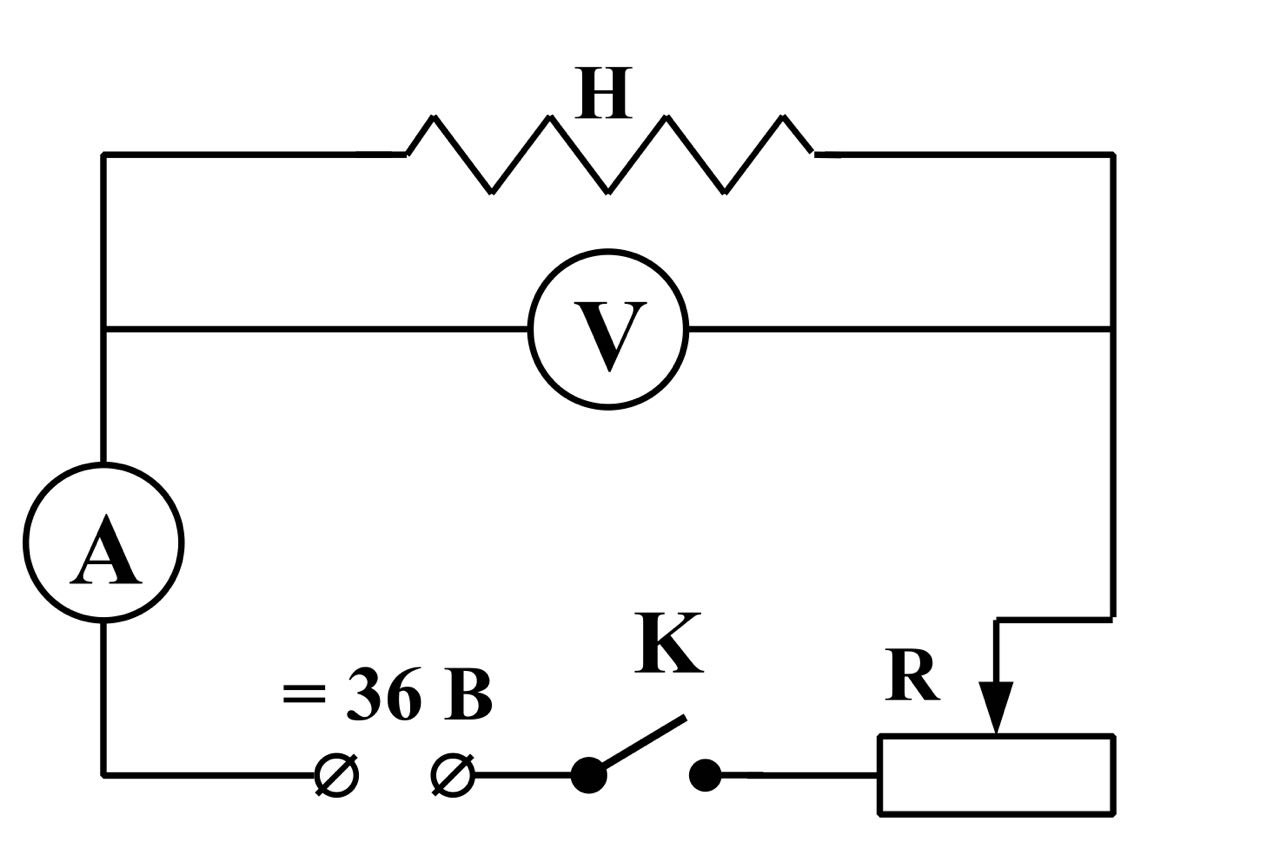
\includegraphics[scale=0.07]{img/schem.jpg}
		\caption{Схема включения нагревателя}
		\label{fig:schem_of_facility}
	\end{center}
\end{wrapfigure}

Установка состоит из калориметра с пенопластовой изоляцией, помещенного в ящик из многослойной клееной фанеры. Внутренние стенки калориметра выполнены из материала с высокой теплопроводностью. Надежность теплового контакта между телом и стенками обеспечивается их формой: они имеют форму усеченных конусов и плотно прилегают друг к другу. Для выталкивания образца служит винт в донышке внутренней стенки калориметра.

В стенку калориметра вмонтированы электронагреватель и термометр сопротивления. Схема включения нагревателя изображена на рисунке (\ref{fig:schem_of_facility}). Система реостатов позволяет установить нужную силу тока в цепи нагревателя. По амперметру и вольтметру определяется мощность, выделяемая током в нагревателе. Величина сопротивления термометра нагревателя  измеряется мостом постоянного тока.

\begin{figure}[h!]
	\begin{center}
		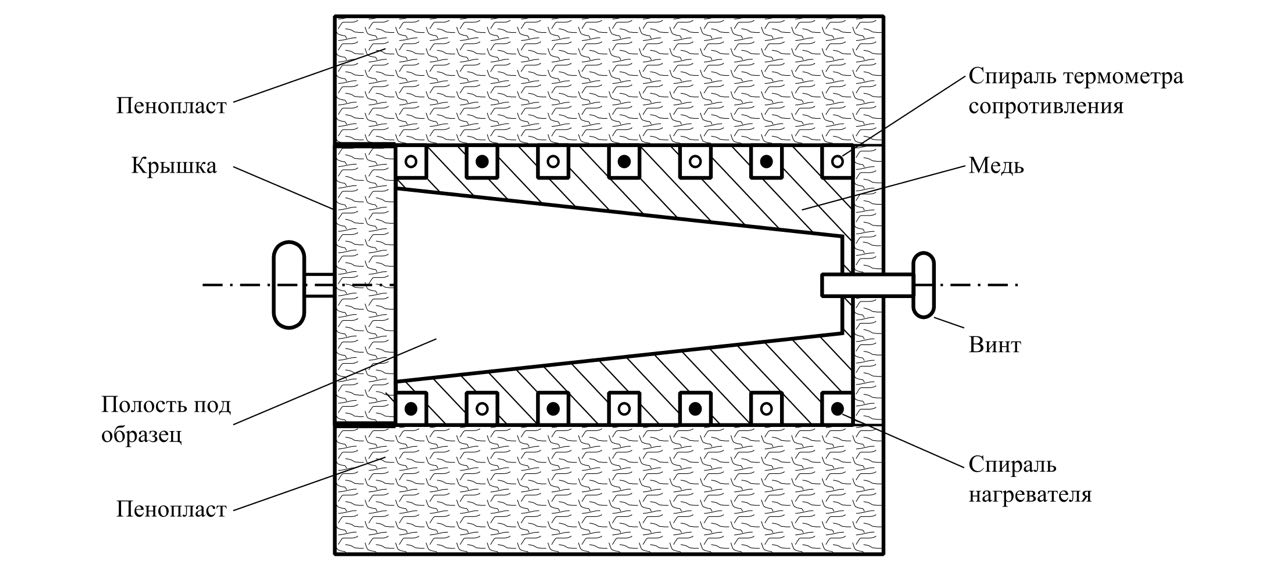
\includegraphics[scale=0.3]{img/ustfig.jpg}
		\caption{Устройство калориметра}
		\label{fig:Ris_of_facility}
	\end{center}
\end{figure}	

На рисунке (\ref{fig:Ris_of_facility}) изображено устройство калориметра.

\begin{center}
	\subsection*{Погрешности}
\end{center}

\begin{itemize}
	\item $\sigma_T = 0,01 ^{\circ}C $
	\item $\sigma_{T_{K}} = 0,01 ^{\circ}C $
	\item $\sigma_U = 0,01 \; \text{В}$
	\item $\sigma_I = 0,0001 \; \text{А}$
	\item $\varepsilon_C = \sqrt{(\frac{\sigma_I}{I})^2 + (\frac{\sigma_T}{T})^2 + (\frac{\sigma_U}{U})^2 + (\frac{\sigma_{T_K}}{T_K})^2} = 3,5 \; \%$
\end{itemize}


\begin{center}
	\section*{Ход работы}
\end{center}


\begin{center}
	Параметры экспериментальной установки:
\end{center}

\begin{table}[h!]
	\centering
	\begin{tabular}{|c|c|}
		\hline
		материал образца: & титан           \\ \hline
		масса образца, г  & $293,2 \pm 0,5$ \\ \hline
	\end{tabular}
	\caption{Параметры исследуемых образцов}
	\label{tab:param_of_facility}
\end{table}

$$R_{0} = 17,84 \pm 0,01 \, \text{Ом}, \quad t_{0} = 21,9^{\circ} \pm 1 ^{\circ} C$$

$$ U = 36 \, \text{В}, \, I = 0,3 \, \text{А}, \, P = 10,8 \, \text{Вт} $$

\centering
Построим графики зависимости $R(t)$ для полученных данных (Рис. 3).

\begin{figure}[ht]

	\subcaptionbox*{Нагрев калориметра}[.45\linewidth]{%
    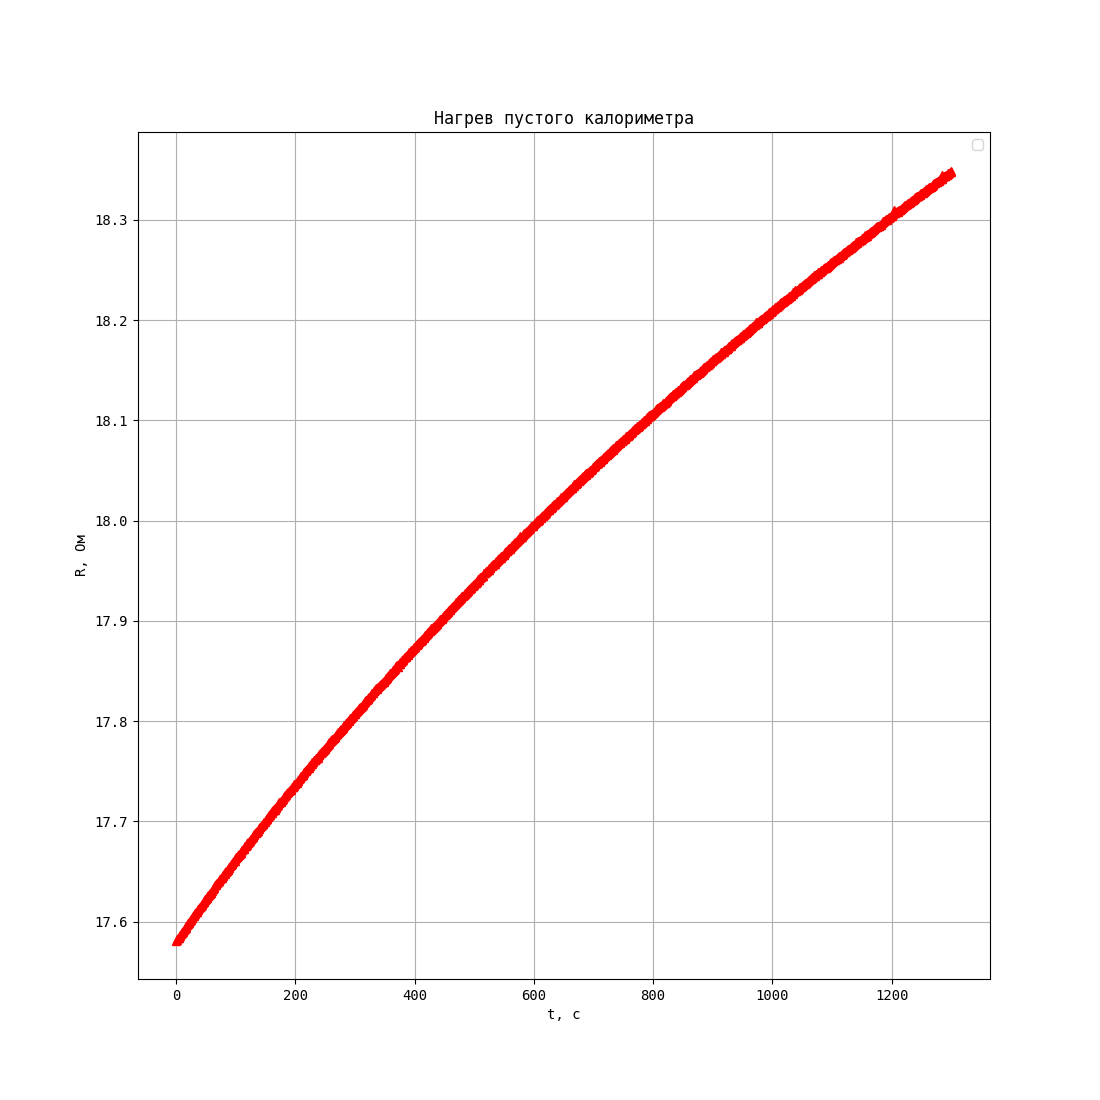
\includegraphics[width=\linewidth]{img/Figure_1.png}%
  }%
  \hfill
  \subcaptionbox*{Нагрев титана}[.45\linewidth]{%
    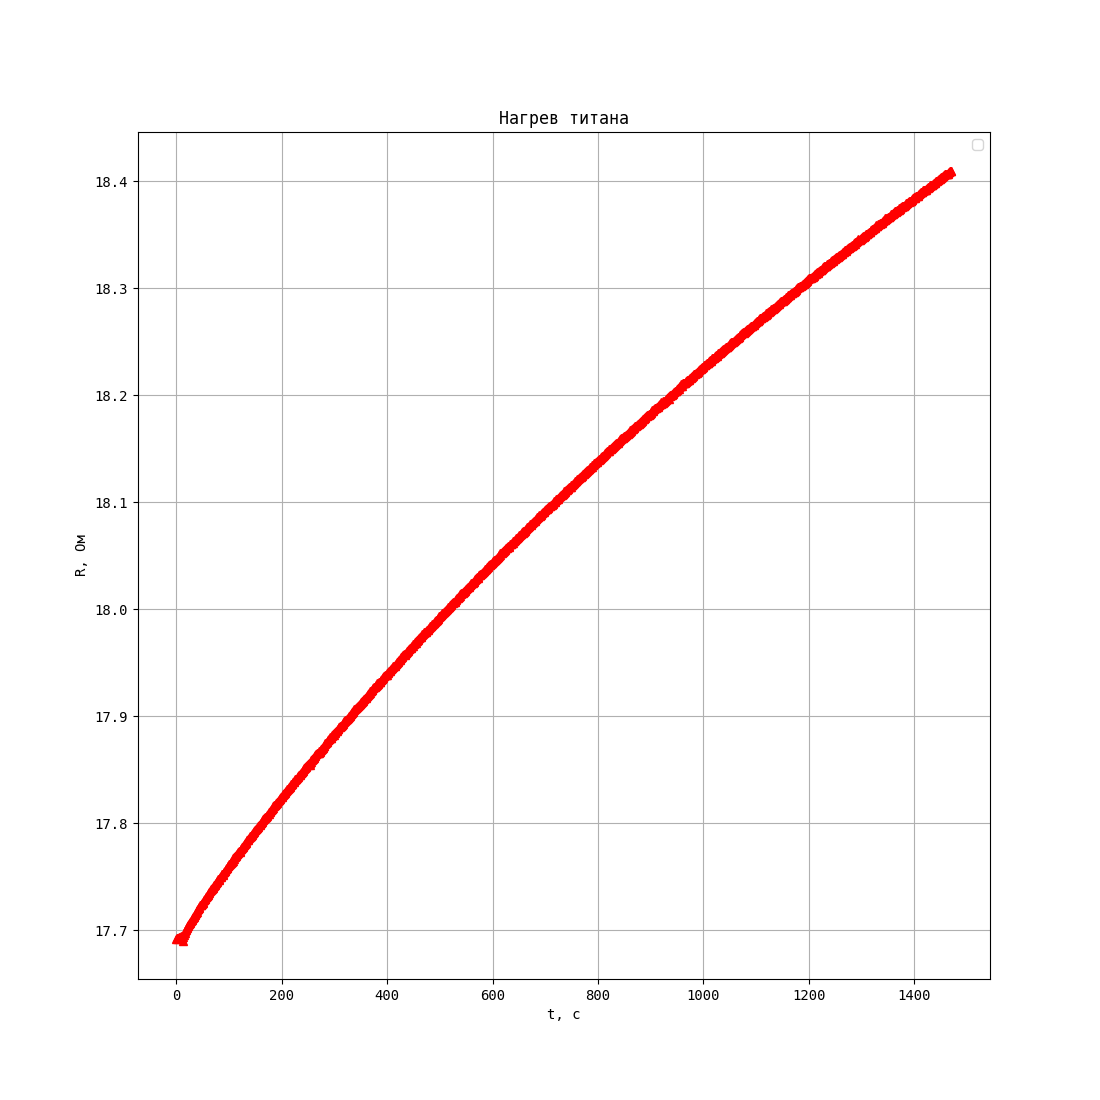
\includegraphics[width=\linewidth]{img/Figure_2.png}%
  }

\end{figure}

Экстраполируем полученные зависимости полиномом второй степени до значений $R = R_{\text{к}}$ и вычислим значения $(\frac{dR}{dt})_{T = T_{\text{к}}}$ с использованием полученной формулы.

\begin{table}[!h]
	\centering
	\begin{tabular}{|l|l|l|l|}
		\hline
		& Уравнение экстраполяции                     & $R_{\text{к}}$, Ом     & $(dR/dt)_{R_{\text{к}}}$, Ом/с     \\ \hline
		Калориметр & $y = -0,0000001x^2 - 0,0008x + 17,589$ & 18,34 & 0,00080 \\ \hline
		Титан      & $y = -0,0000001x^2 - 0,0006x + 17,699$ & 18,41 & 0,00059 \\ \hline
	\end{tabular}
	\caption{Экстраполяция}
\end{table}

Вычисляем теплоемкость по формуле выше:

\begin{table}[H]
	\begin{center}
		\scalebox{0.85}{
		\begin{tabular}{|l|l|l|}
			\hline
			& Теплоемкость, Дж/кг$\cdot$К & Тепл. без калориметра, Дж/кг$\cdot$К \\ \hline
			Калориметр & 212,65  & -                                           \\ \hline
			Титан      & 772,40  & 559,75                   			       \\ \hline
		\end{tabular}}
	\end{center}
	\caption{Результат вычислений теплоемкости}
\end{table}

\begin{center}
	Итого:

\[ \boxed{	C_{\text{титан}} = (559,75 \pm 19,51) \; \frac{\text{Дж}}{\text{кг}\cdot\text{К}}}\quad\]
\end{center}

\begin{center}
	\subsection*{Обсуждение резльтатов}
\end{center}

В пределах погрешности удельная теплоемкость титана $C_{\text{титан}}$ близка к табличному значению $C_{\text{титан}_0} = 523 \frac{\text{кДж}}{(\text{кг}\cdot\text{K})}$

\section*{Выводы}

\begin{itemize}
	\item В ходе работы были измерены теплоемкости калориметра, образца из титана.
	
	\item Основной вклад в (не)точность результата внесла погрешность экстраполяции.
	
	\item Экспериментально проверена работоспособность предложенной методики измерения.
\end{itemize}

\end{document}